\section[时间系统对于GPS的意义]{时间系统对于GPS的意义\\Time Systems Relevant for GPS}

	\subsection[狭义相对论和广义相对论]{狭义相对论和广义相对论\\Special and General Relativity}
		
	GPS定位中相对论效应是为数不多的必须要考虑的日常事件。整个系统是基于时钟的,时钟会发生偏移。
	
	所有的时钟都在地球的引力场中,所以广义相对论是很重要的。时钟信号的标称频率为10.23 MHz。实际上,由于相对论效应的影响,卫星钟准确的频率是10.22999999943 MHz 这样就和用户在地球上的10.23 MHz的频率一致了。
	
	由于卫星时钟相对与接收机时钟是运动的,所以在狭义相对论的情况下时间膨胀了。并且地球一直在旋转,光线跟随着螺旋的路径。我们不能完全同步时钟。
	
	萨尼亚克效应的旋转也是迷人的。它破坏了爱因斯坦的同步,这取决于一个常数的光速。这种恒定性局限于惯性系(无相对加速度)。地球的旋转意味着时钟A可以同步时钟B,时钟B可以同步时钟C,但时钟C不同步时钟A。所以我们需要一个世界时,会以不同的速度同步当地时间。这种协调世界时保持在科罗拉多斯普林斯的GPS控制中心。
	
	\subsection[GPS时间和跳秒]{GPS时间和跳秒\\GPS Time and Leap seconds}
	GPS的基本时间单位是国际单位制(SI)的秒。国际单位制的秒在1967年的第13届的国际计量大会上被定义为“铯原子$Cs^133$基态的两个超精细能级间跃迁辐射振荡9192631170周所持续的时间”。国际单位制的天被定义为84400SI秒,一个儒略世纪是36525(SI)天。
	
	为了弥补真太阳时不均匀的缺陷,人们定义了一个假太阳,其运动轨道位于赤道平面,并且它在赤道上的运动角速度时恒定的。平太阳的时角叫做世界时(UT)。

	儒略日JD日期的表达是一段固定的时间和在基本历元后的部分时间(???)。儒略日的起点为公元前4713年1月1日 $12^h$ 世界时。儒略日时间表示日期是连续计数的,
	
	当前时间用JD表示是一个数值比较大的数,所以使用简化儒略日MJD来代替。
	$$MJD = JD-2 400 000.5.$$
	因此J2000.0(公元2000年) = MJD 51544.5。MJD是以1858年11月17日平子夜作为起点。
	\begin{table}
		\centering
		\caption{UTC和GPST之间的调整日期和跳秒数}
		\label{tab:9.2}
		\begin{tabular}{cc}
			\hline 跳秒数 & 调整日期 \\ 
			\hline  
			1 & 1982-06-30 \\ 
			2 & 1983-06-30 \\ 
			3 & 1985-06-30 \\ 
			4 & 1987-12-31 \\ 
			5 & 1989-12-31 \\ 
			6 & 1990-12-31 \\ 
			7 & 1992-06-30 \\ 
			8 & 1993-06-30 \\ 
			9 & 1994-06-30 \\ 
			10 & 1995-12-31 \\ 
			11 & 1997-06-30 \\ 
			12 & 1998-12-31 \\ 
			13 & 1999-12-31 \\ 
			14 & 2005-12-31 \\ 
			15 & 2008-12-31 \\ 
			\hline 
		\end{tabular} 
	\end{table}
	
	为了在世界范围内保持时间和完整的描述闰秒。国际原子时间尺度(TAI)不与太阳时保持同步,由于地球的自转速度是每年放缓近1s。实现平均太阳时称为世界时(UT1)。协调世界时(UTC)与国际原子时(TAI)由一个整秒数的偏移量定期更新,以保持UTC接近UT1。
	
	跳秒是由IERS(国际地球自转服务)提出的,所以协调世界时(UTC)与世界时(UT1)的时刻差不能大于0.9s。(国际地球自转服务也负责维护的连续性与早期光学仪器采集的数据)DUT1是UT1-UTC的差值,播出的时间信号的精度为$\pm$0.1 s
	
	时间信号由GPS卫星广播,而GPS卫星的时间与GPS主控制站(位于科罗拉多州)的原子钟时间同步。全球定位系统时间GPST的起始时刻为1980年1月6日$0^h$,起始时刻与UTC对齐,但并不增加UTC的闰秒。因此,有一个整秒数的偏移抵消GPST和TAI之间19s的差值。
	$$GPST + 19 s = TAI.$$
	表格\ref{tab:9.2}显示了从1980年1月6日到2011年的所有的15个跳秒。
	$$GPST = UTC + 15 s.$$
	
	随着GPST,从一开始介绍了GPS周数。自1980年1月6日,每周都有自己的编号。这本书写在第1625周。在一周中有了周积秒(sow)的概念。这个数字计数是从周六的午夜开始的,周日是GPS一周的开始。
	
	另外为了方便,每周的每一天有一个数字编号:周日是1,周一是2,周二是3,周三是4,周四是5,周五是6,周六是7。
	
	专业的GPS软件使用周积日(dow)有数值的原因。周积秒(sow)就像这么$7 \times 24 \times 60 \times 60 = 604 800 s$大。为了跟踪一个点的位置(mm级),我们必须保证时间在0.01ns的精度水平。使用周积秒(sow)和12位小数超出了大多数计算机的计算能力。所以你可能将一周内真正的秒数分割成一个整数部分和小数部分或者计算时间的GPS周数,周积日和日积秒。
	
	M文件 $gps\_time$ 用于计算GPS时间 (GPS周(w)和周积秒(sow)):
	\begin{lstlisting} 
	t = julday(2011,3,2,10); % year, month, day, hour
	[w,sow] = gps_time(t)
	w = 1625
	sow = 295200
	\end{lstlisting}
	为了避免在一周的开始和结束时发生低于或高于限制的错误我们使用M文件$check\_t$。
	\subsection[例子1]{例子1\\easy1}\label{subsec:easy1}
	几乎所有GPS的处理都开始自时间问题,\ref{subsec:easy1}展示了如何将一个给出年,月,日,小时,分钟,秒和儒略日的历元时间转化为,GPS周和周积秒(sow)。
	
	下面是sate247j的RINEX格式的观测文件的样本:
	
	\begin{figure}
		\centering
		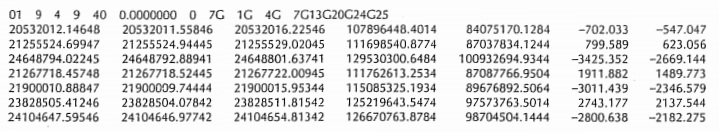
\includegraphics[width=1.0\linewidth]{TeX_files/Part03/chapter09/image/9-site247j}
	\end{figure}
	
	这个数据块的第一行告诉历元时间和有哪些观测到的伪随机噪声卫星。我们解释一下时间是2001年4月9日在9小时40分0秒。随后的0表示接收机处于静态模式;接下来我们读到接收机对7个GPS卫星1、4、7、13、20、24、25进行跟踪。
	
	下面的七行包含七个卫星的伪距和载波观测值有:L1上C/A码所测定的伪距,L1和L2上的P码所测定的伪距,L1和L2上的相位观测值,L1和L2上的多普勒频率。
	
	\subsection[估计接收机时钟偏移量]{估计接收机时钟偏移量\\Estimation of Receiver Clock Offset???}
	现在我们开始使用数据。第一步是估计时钟偏移量$c\,dt_t$。在GPS测量中,观测码$b_t$(伪距)通常被用来估计一个单点的坐标和接收机时钟偏移的顺序(随时间变化)。假设历元时间t提供线性观测值$b_t$:
	
	\begin{equation}\label{eq:9.1}
	A_t 
	\begin{bmatrix}
	x \\	y \\	z
	\end{bmatrix}
	+e_tcdt_t=b_t-\epsilon _t,\qquad t = 1,2,\ldots ,n.
	\end{equation}
	矩阵$A_t$包含t时刻的伪距观测值对坐标的偏导数。后文中式\ref{eq:9.22}。添加每个伪距观测的钟差,$e_t = (1, 1,\ldots ,1 )^T$当该历元有m个卫星时其中便有m项。
	我们收集n个历元的观测值统一成为一个的最小二乘问题
	
	\begin{equation}\label{eq:9.2}
	\begin{bmatrix}
	A_1 \\	A_2 \\	\vdots \\	A_n \\
	\end{bmatrix}
	\begin{bmatrix}
	x \\	y \\	z 
	\end{bmatrix}
	+		
	\begin{bmatrix}
	e_1 & & & \\
	& e_2 & & \\	
	& & \ddots & \\	
	& & & e_n  
	\end{bmatrix}
	\begin{bmatrix}
	c\,dt_1 \\	
	c\,dt_2 \\	
	\vdots \\	
	c\,dt_n
	\end{bmatrix}
	=\begin{bmatrix}
	b_1 \\ b_2 \\ \vdots \\ b_n
	\end{bmatrix}
	-
	\epsilon
	\end{equation}
	\begin{figure}
		\centering
		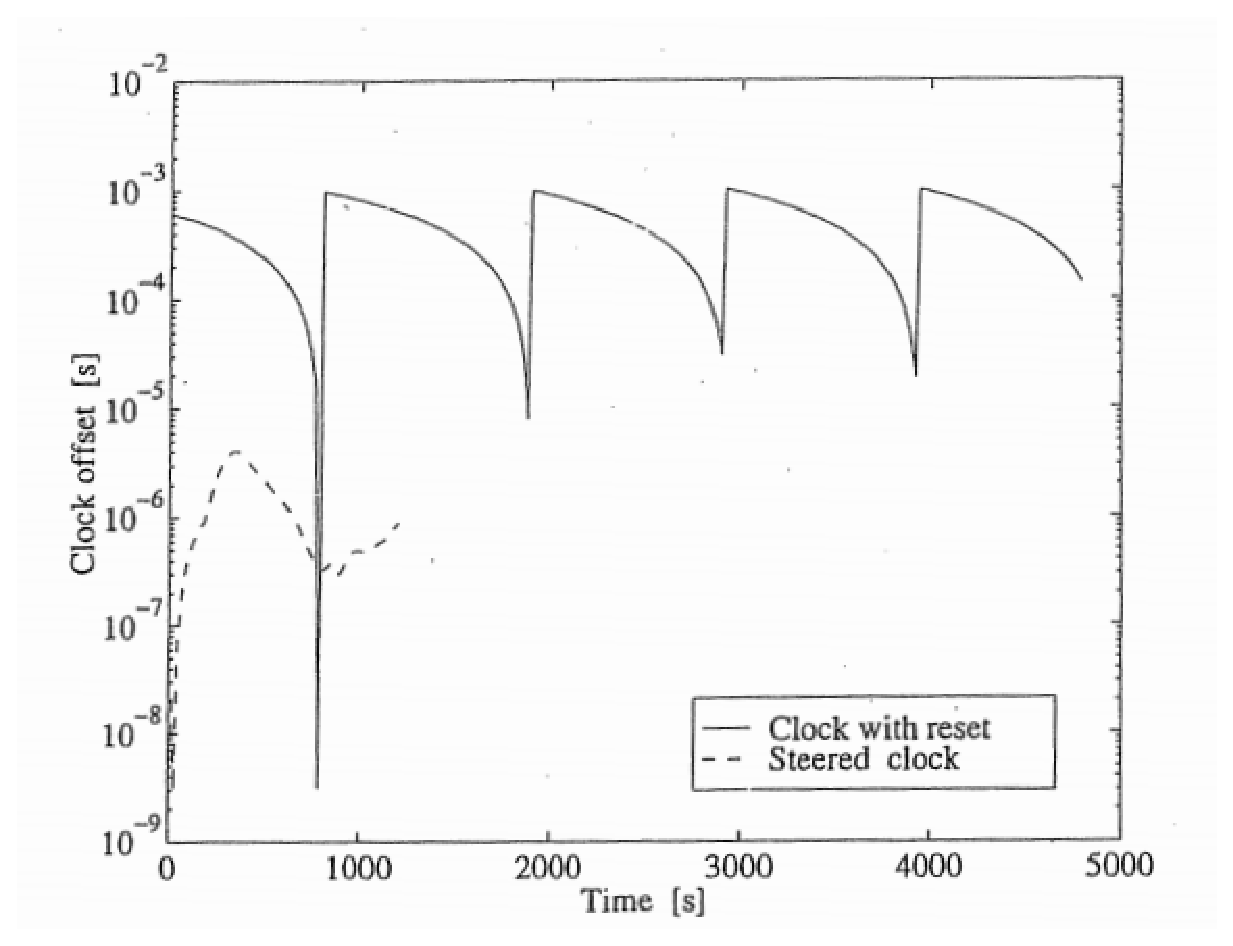
\includegraphics[width=0.7\linewidth]{TeX_files/Part03/chapter09/image/9-4}
		\caption{不同类型接收机的时钟偏移量。时钟重置时间为1ms。}
		\label{fig:9-4}
	\end{figure}
	
	正规方程组\ref{eq:9.2}通过最小二乘方法获得最优的$x,y,z,c\,dt_t$解。
	
	\begin{equation}\label{eq:9.3}
	\begin{bmatrix}
	e^T_1e_1 & & & & e^T_1A_1 \\
	& e^T_2e_2 & & & e^T_2A_2 \\
	& & \ddots   & & \vdots	  \\
	& & & e^T_ne_n & e^T_nA_n \\
	A^T_1e_1 & A^T_2e_2 & \ldots & A^T_ne_n & \Sigma ^n_{t=1}A^T_tA_t
	\end{bmatrix}
	\begin{bmatrix}
	c\,dt_1 \\
	c\,dt_2 \\
	\vdots
	c\,dt_n \\
	x \\
	y \\
	z 
	\end{bmatrix}
	=
	\begin{bmatrix}
	e^T_1b_1 \\
	e^T_2b_2 \\
	\vdots	 \\
	e^T_nb_n \\
	\Sigma ^n_{t=1}A^T_tb_t
	\end{bmatrix}
	\end{equation}
	
	使用普通高斯消元法从n个方程中消去n倍的最后一行。我们写下$E_t$矩阵$e_t(e^T_te_t)^{-1}e^T_t$ 。修正(x,y,z)坐标到初步位置(x°,y°,z°)是由矩阵右下角出现的项来消除的。根据式\ref{eq:6.46}。
	$$x=\begin{bmatrix}
	x \\ y \\ z
	\end{bmatrix}=\left( \sum^n_{t=1}(A^T_tA_t-A^T_tE_tA_t)\right)^{-1}\sum^n_{t=1}(A^T_tb_t-A^T_tE_tb_t) $$
	估计接收机时钟偏移量 $c\,dt_t$是通过回代法解决,$i=n,\ldots,1$:
	\begin{equation}
	c\,dt_t=(e_tb_t-e_tA_tx)/(e_te_t^T).
	\end{equation}
	
	估计模型清楚地显示为什么没有必要为所有历元的静态观测收集四个观测值。但需要足够数量的观测值来保持\ref{eq:9.3}是可逆的。如果只有一个观测值是可以在一个特定的历元估计接收机时钟偏移,但不能估计位置。
	\begin{figure}
		\centering
		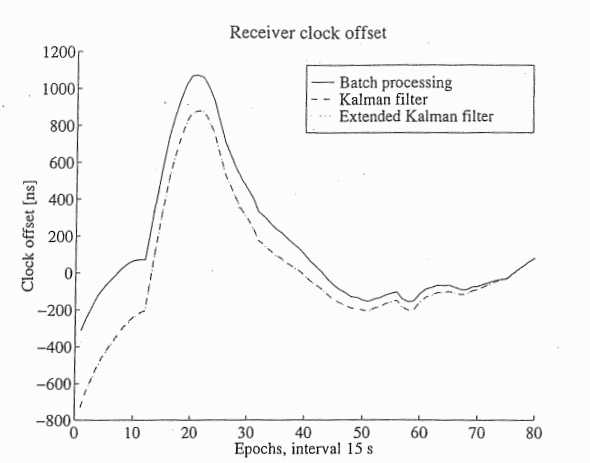
\includegraphics[width=0.7\linewidth]{TeX_files/Part03/chapter09/image/9-5}
		\caption{接收机时钟偏移计算的批处理和卡尔曼滤波。普通和扩展卡尔曼滤波的线性方程}
		\label{fig:9-5}
	\end{figure}
	
	我们建议使用描述程序,一些制造商引入不连续的时钟时间变化以保证误差在规定的补偿要求内。某些接收机时钟在复位时抵消1毫秒。图\ref{fig:9-4}展示了这种跳跃方式抵消钟差的接收机类型,以及这种类型的接收机如何操纵时钟。
	
	图\ref{fig:9-5}显示了接收机时钟偏移量与不断修正以抵消的操纵方式。图像是由M文件recclock提供。代码迭代三次得到正确的接收机位置——时钟估计是线性的!
	
	\subsection[例子7]{例子7\\easy7}\label{subsec:easy7}
	伪距这个词的“伪”部分暗指接收机时钟偏移dt。常常dt是一个不太关心的参数。然而在某些情况下需要知道dt。我们应用该算法(9.4)来获取dt。
	
	实际数据产生$dt\approx0.38 ms$ 如图\ref{fig:9-6}所示。可以看到接收机时钟的速率是在很短的时间内相当稳定。
